%%%%%%%%%%%%%%%%%%%%%%%%%%%%%%%%%%%%%%%%%%  不使用 authblk 包制作标题  %%%%%%%%%%%%%%%%%%%%%%%%%%%%%%%%%%%%%%%%%%%%%%
%-------------------------------PPT Title-------------------------------------
\title{{\rm LAMMPS}算例举要}
%-----------------------------------------------------------------------------
%----------------------------Author & Date------------------------------------

%\author[\textrm{Jun\_Jiang}]{姜\;\;骏\inst{}} %[]{} (optional, use only with lots of authors)
%% - Give the names in the same order as the appear in the paper.
%% - Use the \inst{?} command only if the authors have different
%%   affiliation.
\institute[BCC]{\inst{}%
%\institute[Gain~Strong]{\inst{}%
\vskip -20pt 北京市计算中心~云平台事业部~~姜骏}
%\vskip -20pt {\large 格致斯创~科技}}
\date[\today] % (optional, should be abbreviation of conference name)
{%	{\fontsize{6.2pt}{4.2pt}\selectfont{\textcolor{blue}{E-mail:~}\url{jiangjun@bcc.ac.cn}}}
\vskip 45 pt {\fontsize{8.2pt}{6.2pt}\selectfont{%清华大学\;\;物理系% 报告地点
	\vskip 5 pt \textrm{2023.11.23-24}}}
}

%% - Either use conference name or its abbreviation
%% - Not really information to the audience, more for people (including
%%   yourself) who are reading the slides onlin%%   yourself) who are reading the slides onlin%%   yourself) who are reading the slides onlineee
%%%%%%%%%%%%%%%%%%%%%%%%%%%%%%%%%%%%%%%%%%%%%%%%%%%%%%%%%%%%%%%%%%%%%%%%%%%%%%%%%%%%%%%%%%%%%%%%%%%%%%%%%%%%%%%%%%%%%

\subject{}
% This is only inserted into the PDF information catalog. Can be left
% out.
%\maketitle
\frame
{
%	\frametitle{\fontsize{9.5pt}{5.2pt}\selectfont{\textcolor{orange}{“高通量并发式材料计算算法与软件”年度检查}}}
\titlepage
}
%-----------------------------------------------------------------------------

%------------------------------------------------------------------------------列出全文 outline ---------------------------------------------------------------------------------
\section{基本计算}\label{Sec:General}
%真空中的孤立原子的基态能量是\textrm{VASP}中最简单的算例,通过学习金属\textrm{Pt}原子基态能量的计算,可以掌握典型的\textrm{VASP}的主体流程\footnote{在所有计算之前,请确认\textrm{VASP}软件已经正确安装。},了解体系基态能量最小化的基本算法,并熟悉基本的输入/输出文件的内容。此外,还可以了解如何在已完成计算的基础上,进行计算精度提升或完成后续计算等一系列处理方式。
%\subsection{输入文件}
\frame
{
	\frametitle{\textrm{LAMMPS}一般计算流程}
\begin{figure}[h!]
\centering
\vskip -5pt
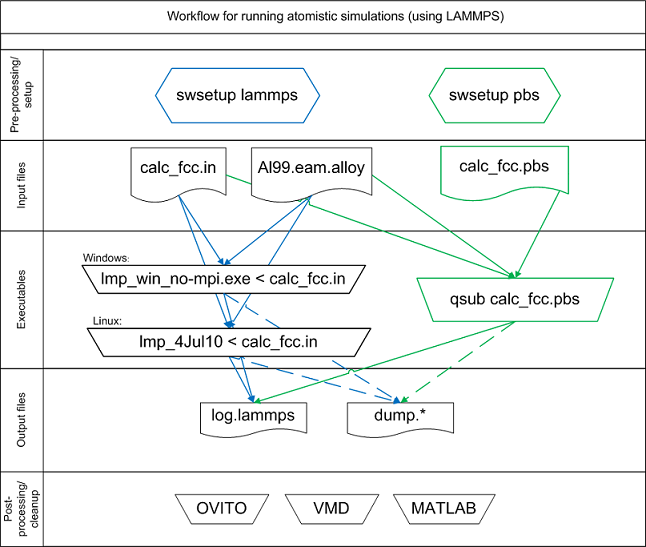
\includegraphics[height=2.50in,width=3.0in, viewport=0 0 646 547,clip]{Lammps_workflow.png}
\caption{\fontsize{6.2pt}{5.2pt}\selectfont{\textrm{The general workflow for running molecular dynamics simulations using LAMMPS.}}}%(与文献\cite{EPJB33-47_2003}图1对比)
\label{General_Workflow}
\end{figure}
}

\frame[allowframebreaks]
{
	\frametitle{\textrm{LAMMPS}的输入文件}
\fontsize{6.0pt}{4.0pt}\selectfont{
%\verbatiminput{Figures/Lammps_in_lj.txt} %为保险:~选用文件名绝对路径
\verbatiminput{Figures/Lammps_tutorial-01-in.txt} %为保险:~选用文件名绝对路径
}
}

\frame
{
	\frametitle{\textrm{LAMMPS}的输出结果}
\begin{figure}[h!]
\centering
\vskip -5pt
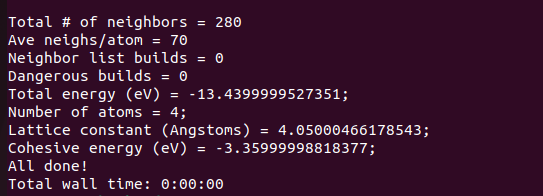
\includegraphics[height=1.50in,width=4.0in, viewport=0 0 543 196,clip]{Lammps_output.png}
\caption{\fontsize{6.2pt}{5.2pt}\selectfont{\textrm{The end of the logfile/screen output using LAMMPS.}}}%(与文献\cite{EPJB33-47_2003}图1对比)
\label{LAMMPS_output}
\end{figure}
}

%\frame
%------------------------------------------------------------------------Reference----------------------------------------------------------------------------------------------
		\frame[allowframebreaks]
{
\frametitle{主要参考文献}
\begin{thebibliography}{99}
{\tiny
	\bibitem{J.-G._Lee}\textrm{J.-G. Lee, \textit{Computational Materials Science:~an introduction}}~\textrm{(2nd Edition),~CPC Press}, \textrm{(2017)}
	\bibitem{VASP_tutorial}\url{https://www.vasp.at/wiki/index.php/Category:Examples}
	\bibitem{Comp_Phys}\textrm{J. M. Thijssen. \textit{Computational Physics}~\textrm{(2nd Edition)} (Cambridge University Press, Cambridge, England, 2007)}
	\bibitem{PRB78-205302_2008}\textrm{H. Bentmann and A. A. Demkov and R. Gregory and S. Zollner. \textit{Phys. Rev. B} \textbf{78} (2008), 205302}
	\bibitem{Landolt-Bornstein}\textrm{Landolt-B\"ornstein, \textit{Structure Data of Elements and Intermetallic Phase},~Springer Inc.}, \textrm{(1991)}
	\bibitem{PSSA102-47_1987}\textrm{H. E. Sch\"afer. \textit{Phys. Status Solidi A} \textbf{102} (1987), 47}
	\bibitem{PRB66-214110_2002}\textrm{T. R. Mattson and A. E. Mattson. \textit{Phys. Rev. B} \textbf{66} (2002), 214110}
	\bibitem{JNM383-244_2009}\textrm{S.-C. Lee, J.-H. Choi and J. G. Lee. \textit{J. Nuclear Mat.} \textbf{383} (2009), 244}
	\bibitem{JMS44-1828_2009}\textrm{J. H. Kim, Y. D. Kwon, P. Yonathan,I. Hidayat,J. G. Lee, J.-H. Choi and S.-C. Lee. \textit{J. Matt. Sci.} \textbf{44} (2009), 1828}
	\bibitem{Electrochim52-2219_2007}\textrm{M. C. Lischka, C Mosch and A. Gro$\beta$. \textit{Electrochim. Acta..} \textbf{52} (2007), 2219}
	\bibitem{url_plot-workfunc}\url{https://gist.github.com/Ionizing/1ac92f98e8b00a1cf6f16bd57694ff03}
	\bibitem{Phonopy}\url{http://phonopy.sourceforge.net/}
	\bibitem{PRB52-R5467_1995}\textrm{A. I. Liechtenstein, V. I. Anisimov and J. Zaanen., \textit{Phys. Rev.} B, \textbf{52} (1995), R5467}
	\bibitem{PRB57-1505_1998}\textrm{S. L. Dudarev, G. A. Botton, S. Y. Savrasov, C. J. Humphreys and A. P. Sutton., \textit{Phys. Rev.} B, \textbf{57} (1998), 1505}
	\bibitem{PRB73-045112_2006}\textrm{M. Gajdo$\check{s}$, K. Hummer, G. Kresse, J. Furthm\"uller and F. Bechstedt. \textit{Phys. Rev.} B, \textbf{73} (2006), 045112}
}
\end{thebibliography}
}
